\documentclass[twocolumn,compsoc,journal,demo]{IEEEtran}
\usepackage{graphicx}
%\usepackage[caption=false,font=normalsize,
%labelfont=sf,textfont=sf]{subfig}
\usepackage[font=normalsize,labelfont=sf,textfont=sf]{subcaption} % Use only subcaption, not subfig

\begin{document}
	
	\begin{figure*}
		\centering % 将整个 figure* 居中
		\begin{minipage}[b]{\columnwidth}
			\subfloat[]{
\includegraphics[width=\columnwidth,height=\columnwidth]{Tsinghua_University_Logo-eps-converted-to.pdf}}
		\end{minipage}
		\hfill
		\begin{minipage}[b]{\columnwidth}
			\subfloat[]{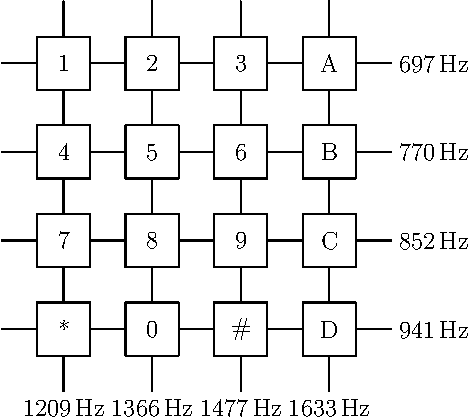
\includegraphics[width=.475\linewidth]{dtmf.pdf}}
			\hfill 
			\subfloat[]{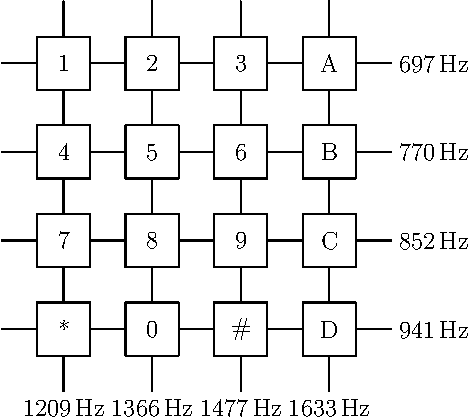
\includegraphics[width=.475\linewidth]{dtmf.pdf}}
			
			\subfloat[]{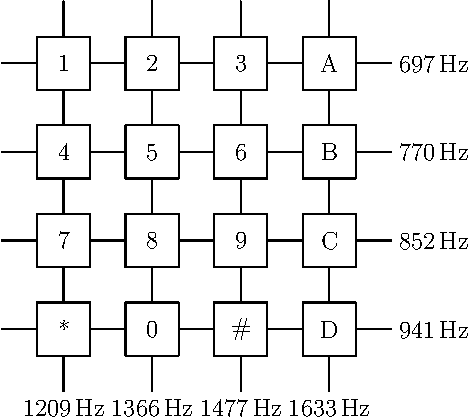
\includegraphics[width=.475\linewidth]{dtmf.pdf}}
			\hfill 
			\subfloat[]{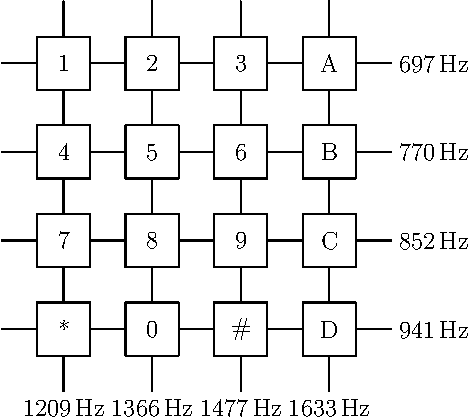
\includegraphics[width=.475\linewidth]{dtmf.pdf}}
		\end{minipage}
		\caption{Sparsity Structure of some sparse matrices}
		\label{freq} 
	\end{figure*} 
	
	\begin{figure}
		\centering % 将整个 figure 居中
		\begin{subfigure}{0.45\linewidth}
			\includegraphics[width=\linewidth]{example-image-a}
			\caption{Subfigure A}
			\label{subfig:a}
		\end{subfigure}
		\hfill
		\begin{subfigure}{0.45\linewidth}
			\includegraphics[width=\linewidth]{example-image-b}
			\caption{Subfigure B}
			\label{subfig:b}
		\end{subfigure}
		\caption{Caption Title}
		\label{fig:subfigures}
	\end{figure}
\end{document}
